\problemname{Pýramídasala}
\illustration{0.3}{pyramid}{Mynd fengin af \href{https://flic.kr/p/sfeE3r}{flickr.com}}

Fyrirtækið Pýramídar ehf.\ selur hundruði pýramída hvert ár.
Viðskiptamódelið þeirra er frábrugðið því sem þekkist almennt hjá fyrirtækjum.
Pýramídas, eigandi fyrirtækisins, réði starfsmenn sem selja fyrir fyrirtækið.
Starfsmenn Pýramídasar ráða svo sína eigin starfsmenn, þeirra starfsmenn ráða 
sína eigin starfsmenn, og svo framvegis.
Starfsmenn eru því með einn yfirmann (nema Pýramídas) en geta haft marga undirmenn.
Ef að starfsmaður er með undirmann þá mun hann alltaf hafa að
minnsta kosti tvo undirmenn.
Í öðrum orðum, þá mun starfsmaður aldrei hafa nákvæmlega einn undirmann.
Athugið að undirmönnum er raðað eftir því hvenær þeir voru ráðnir;
undirmaðurinn sem var ráðinn fyrst kemur fremst, sá næsti á eftir honum, og svo
framvegis.

Pýramídas á alla pýramídana í upphafi og selur þá áfram til starfsmanna sinna.
Þeir selja svo pýramídana áfram til starfsmanna sinna og heldur það áfram
þar til pýramídarnir eru komnir í hendur þeirra sem hafa enga starfsmenn undir sér.
Þeir starfsmenn selja pýramídana til þeirra sem eru ekki starfsmenn fyrirtækisins
en hafa samt áhuga á pýramídum.
Starfsmenn þurfa svo að skila $10\%$ af gróða sínum til yfirmanns síns.

Nýlega hafa borist kvartanir um lögmæti starfseminnar.
Þú hefur verið ráðinn til að rannsaka.
Fyrsta skref rannsóknarinnar er að skilja uppbyggingu fyrirtækisins.
Því miður vill enginn starfsmaður veita þér neinar upplýsingar um hverjir starfa
fyrir hvern eða hver sé yfirmaður hvers.

Þú hefur starfsmannaskrá sem segir þér starfsmannanúmer hvers og eins starfsmanns.
Þú hefur einnig komist yfir þrjár runur af starfsmannanúmerum sem eiga að lýsa
uppbyggingu fyrirtækisins.
Vinur þinn Bjarki er sérfræðingur í dulkóðun og hefur komist að því að
eftirfarandi þrjár mismunandi aðferðir voru notaðar til að búa til runurnar
þrjár:

\begin{enumerate}
    \item Fyrst skrifar starfsmaður númerið sitt og skipar undirmönnum sínum að
          fylgja aðgerðum sínum. Undirmenn skipa sínum undirmönnum áfram.
    \item Fyrst skipar hann fyrsta undirmanni sínum að fylgja aðgerðum sínum.
          Næst skrifar hann númerið sitt.
          Þá skipar hann öðrum undirmanni að fylgja aðgerðum sínum.
          Svo skrifar hann númerið sitt.
          Þá er röðin komin að þriðja undirmanni.
          Alltaf skrifar hann númer sitt á milli aðgerða undirmanna sinna þar 
          til síðasti undirmaðurinn hefur klárað.
          Ef starfsmaður hefur engan undirmann þá skrifar hann númer sitt einu sinni.
    \item Fyrst skipar starfsmaður undirmönnum sínum að fylgja aðgerðum sínum og 
          svo skrifar hann númerið sitt. Undirmenn skipa sínum undirmönnum áfram.
\end{enumerate}

Útfrá þessum þremur runum geturðu sagt hver uppbygging fyrirtækisins er?
Hver vinnur fyrir hvern og í hvaða röð voru undirmennirnir ráðnir?

\section*{Inntak}
Inntak er fjórar línur.
Fyrsta línan í inntakinu samanstendur af tveimur heiltölum $1 \leq N \leq 10^{5}$, fjöldi starfsmanna, og $M$, fjöldi talna í runu 2.
Önnur lína samanstendur af $N$ heiltölum, runu 1.
Þriðja lína samanstendur af $M$ heiltölum, runu 2.
Fjórða lína samanstendur af $N$ heiltölum, runu 3.

Starfsmannanúmer eru alltaf heiltölur á bilinu $1$ upp í $N$, en þeim er ekki
úthlutað á neinn sérstakan hátt.

\section*{Úttak}
Skrifið út $N$ línur.
Lína $i$ skal innihalda starfsmannanúmer allra undirmanna starfsmannsins með
númerið $i$, á sama sniði og í sýnidæmunum hér að neðan.

Þið getið gert ráð fyrir að það sé alltaf til nákvæmlega ein lausn.

\section*{Stigagjöf}
\begin{tabular}{|l|l|l|}
\hline
Hópur & Stig & Takmarkanir \\ \hline
1     & 15   & $1 \leq N \leq 100$, starfsmenn hafa í mesta lagi 2 undirmenn og runa 2 er í hækkandi röð \\ \hline
2     & 15   & $1 \leq N \leq 100$ og starfsmenn hafa í mesta lagi 2 undirmenn \\ \hline
3     & 15   & $1 \leq N \leq 100$ \\ \hline
4     & 20   & Starfsmenn hafa í mesta lagi 2 undirmenn og runa 2 er í hækkandi röð \\ \hline
5     & 20   & Starfsmenn hafa í mesta lagi 2 undirmenn \\ \hline
6     & 15   & Engar frekari takmarkanir\\ \hline
\end{tabular}

\section*{Útskýring á sýnidæmum}
Fyrsta sýnidæmið fellur undir hóp 1 og má sjá uppbyggingu fyrirtækisins á myndinni að neðan.

\begin{figure}[h!]
  \centering
    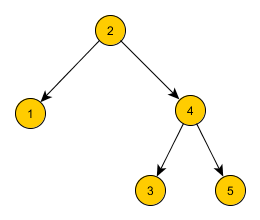
\includegraphics[width=0.5\textwidth]{sample1}
  \caption{Sýnidæmi 1}
\end{figure}

Annað sýnidæmið fellur undir hóp 2 og má sjá uppbyggingu fyrirtækisins á myndinni að neðan.
\begin{figure}[h!]
  \centering
    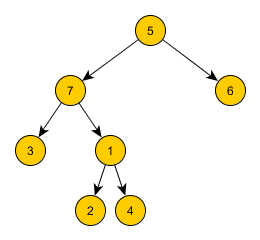
\includegraphics[width=0.5\textwidth]{sample2}
  \caption{Sýnidæmi 2}
\end{figure}

Þriðja sýnidæmið fellur undir hóp 3 og má sjá uppbyggingu fyrirtækisins á myndinni að neðan.
\begin{figure}[h!]
  \centering
    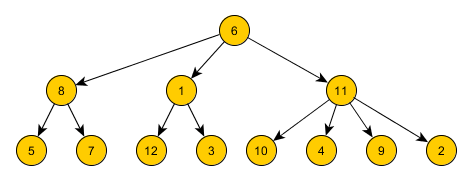
\includegraphics[width=0.5\textwidth]{sample3}
  \caption{Sýnidæmi 3}
\end{figure}
